
%===== Lecture de tension des modules =====

\section{Lecture de tension des modules}
			\subsection{Objectifs}
				Nous d\'{e}sirons avoir une lecture tr\`{e}s pr\'{e}sise (+/- 2mV) du modules. Afin de pouvoir brancher les modules dans n'importe quel ordre sur le BMS, nous devons faire en sorte que les lectures de tension sont isol\'{e}es.Le circuit doit consommer un minimum de courant puisqu'il sera aliment\'{e} par le modules.
			\subsection{Circuit analogique}
				\subsubsection{Sch\'{e}ma}
				\begin{center}
					% Schema
					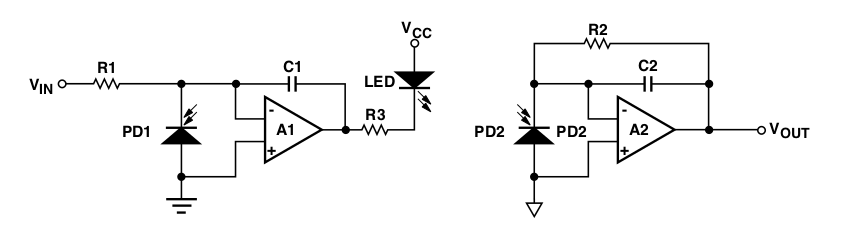
\includegraphics[scale=0.5]{Analog} \\ \vspace{0cm}
				\end{center}
			
				\subsubsection{Analyse}
					%  BOM
					\begin{table}[h!]	
						\centering
						\begin{tabular}{|c|c|c|}
							\hline
							Part number & Description & Prix (total)\\ \hhline{|=|=|=|}
							BU7421SG-TR & Op-amp (2x) & 2\$ \\ \hline
							LOC110STR & Optocoupleur lin\'{e}aire & 4.09\$ \\ \hline
							 \multicolumn{2}{|c|}{*Prix de digikey pour 1 unit\'{e} }& 6.09\$ \\ \hline
						\end{tabular}
						\caption{Bill of material - Analog}
						\label{Table:1}
					\end{table}
						
					% Avantage // Desavantage	
					\begin{table}[h!]
					\centering
						\begin{tabular}{|c|c|}
							\hline
							Avantage & D\'{e}savantage\\ \hhline{|=|=|}
							Peu de composantes & Pr\'{e}cision de +/- 1\% \\ \hline
							Robuste & L'optocoupleur lin\'{e}aire est gros (SOIC 8)\\ \hline
							 & Consomme beaucoup de courant (10mA max)\\ \hline
						\end{tabular}
						\caption{Avantage et d\'{e}savantage - Analog}
						\label{Table:2}
					\end{table} 
					
				\subsubsection{Conclusion}
				% Conclusion
				Le circuit analogique autour de l'optocoupleur lin\'{e}aire n'est pas assez pr\'{e}cis pour \^{e}tre consid\'{e}r\'{e} comme viable pour le projet.De plus, il consomme beaucoup trop de courant pour pouvoir \^{e}tre toujours en marche. Il faudrait ajouter un circuit pour d\'{e}sactiver la lecture lorsqu'elle n'est pas utilis\'{e}. Ceci enl\`{e}ve l'avantage d'utiliser cette solution. 
				\newpage
				
			\subsection{Circuit digital}
				\subsubsection{Protocole de communication}
					Les ADC externes utilisent souvent les m\^{e}me trois interface de communication s\'{e}riel : UART,I2C et SPI. Puisque nous avons un nombre limit\'{e} de ces periph\'{e}rique sur le microcontr\^{o}leur, nous aurons besoin d'un bus qui permet d'avoir un maximum d'ADC. Il nous reste donc le choix entre le I2C et le SPI. Le SPI demanderais d'avoir un circuit d'isolation consid\'{e}rablement plus gros et dispendieux que le I2C. Le SPI \`{a} deux fils de plus que le I2C ( 1 pour le data et 1 pour choisir le "slave"). \\
					Le protocol choisis est le I2C et le circuit d'isolation est le ISO1541DR. Malheureusement, le circuit consomme un petit peu moins de 5mA. Nous devrons donc avoir une alimentation qui permettra de d\'{e}sactiver l'alimentation du c\^{o}t\'{e} du modules lorsque le syst\`{e}me ne sera pas en marche.
					
				\subsubsection{Lecture d'un voltage de r\'{e}f\'{e}rence}
					La premi\`{e}re solution envisag\'{e} \'{e}taient de lire un voltage de r\'{e}f\'{e}rence avec le ADC. Puisqu'on connait la tension \`{a} l'entr\'{e}e, il est possible de d\'{e}terminer la tension de l'alimentation du ADC avec la valeur de la lecture. Le ADS1013 avait \'{e}t\'{e} retenue puisqu'il a une alimentation de 2 \`{a} 5.5V, un quiescent current de 150$\mu$A et une r\'{e}solution de 12 bits. Cependant, ce ADC a une entr\'{e}e diff\'{e}rentielle et nous aurions seulement utilis\'{e} la moiti\'{e}e de la plage. Nous nous retrouverions ainsi avec uns r\'{e}solution de 11 bits. En utilisant un voltage de r\'{e}f\'{e}rence de 2.048V, nous obtenerions une pr\'{e}cision de 4.2mV lorsque le module est \`{a} 4.2V.Nous somme pr\`{e}s de nos objectifs mais le voltage minimum pour l'alimentation de l'isolateur I2C (3V) fait en sorte que cette solution ne peut \^{e}tre envisag\'{e}e.
					% Schema
					\begin{figure}[h]
						\centering
						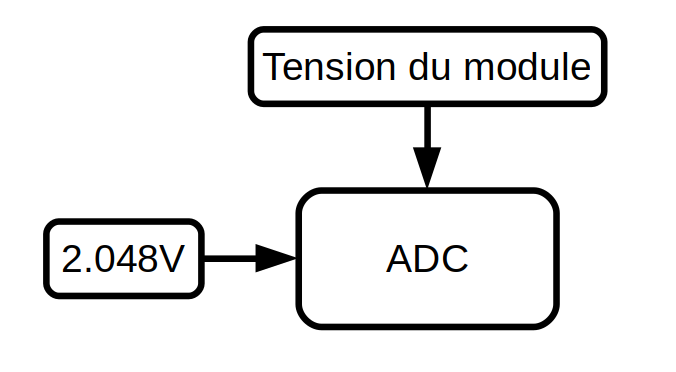
\includegraphics[scale=0.3]{Voltage_reference} \\ \vspace{0cm}
						\caption{Sch\'{e}ma fonctionnel : Voltage de r\'{e}f\'{e}rence }
						\label{fig:schema_voltage_ref}
					\end{figure}

				\newpage
				\subsubsection{Lecture de la tension du module}
					Pour pouvoir mesurer la tension du module, l'alimentation du ADC doit \^{e}tre au dessus du voltage maximal du module plus une marge de s\'{e}curit\'{e}. De plus, il est plus int\'{e}ressant d'utiliser un ADC "single ended" ou "pseudo differential" pour avoir acc\`{e}s \`{a} toute la plage. Il est donc n\'{e}cessaire d'avoir un "boost" pour amener la tension d'alimentation \`{a} 5V. Cette tension va alimenter le circuit d'isolation I2C. Un r\'{e}gulateur lin\'{e}aire sera n\'{e}cessaire pour alimenter le ADC afin d'avoir un minimum de bruit dans les lecture. Un "boost" avec l'option "shutdown" sera utilis\'{e} pour que le circuit ne vide pas les batteries lorsque le "battery pack" est entrepos\'{e}. Un premier ADC, le MCP3221A5T avait \'{e}t\'{e} selectionn\'{e} mais il fut rejet\'{e} puisqu'il est impossible de changer l'adresse du IC (elle doit \^{e}tre chang\'{e} par la compagnie). En ce moment, les pi\`{e}ces envisag\'{e}es sont : \\
					
					%  BOM
					\begin{table}[H]
						\centering
						\begin{tabular}{|c|c|c|}
							\hline
							Part number & Description & Prix (total) \\ \hhline {|=|=|=|}
							ADC121C021CIMM/NOPB & ADC 12 bit I2C & 4.3\$ \\ \hline
							AP2202K-ADJTRG1 & LDO & 0.63\$ \\ \hline
							AP3015KTR-G1 & Boost & 1.1\$ \\ \hline
							ISO1541DR & Isolation I2C & 6.67\$ \\ \hline
							LTV-816S & Optocoupleur (boost shutdown) & 0.61\$ \\ \hline
							\multicolumn{2}{|c|}{ }& 13.31\$ \\ \hline
							\multicolumn{3}{r}{ } Prix de digikey pour 1 unit\'{e} \\ 
						\end{tabular} \\ \vspace{0cm} 
						\caption{Bill of material - Digital}
						\label{Table:3}
					\end{table}
				% Schema
				\begin{figure}[h]
					\centering
					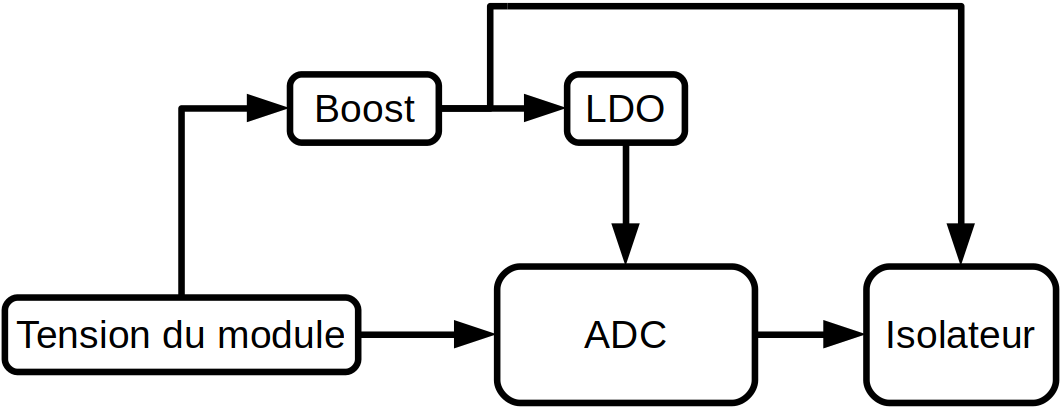
\includegraphics[scale=0.3]{Tension_module} \\ \vspace{0cm}
					\caption{Sch\'{e}ma fonctionnel : Lecture de la tension du module}
					\label{fig:schema_tension_module}
				\end{figure}